\documentclass[10pt]{article}\usepackage[]{graphicx}\usepackage[]{color}
% maxwidth is the original width if it is less than linewidth
% otherwise use linewidth (to make sure the graphics do not exceed the margin)
\makeatletter
\def\maxwidth{ %
  \ifdim\Gin@nat@width>\linewidth
    \linewidth
  \else
    \Gin@nat@width
  \fi
}
\makeatother

\definecolor{fgcolor}{rgb}{0.345, 0.345, 0.345}
\newcommand{\hlnum}[1]{\textcolor[rgb]{0.686,0.059,0.569}{#1}}%
\newcommand{\hlstr}[1]{\textcolor[rgb]{0.192,0.494,0.8}{#1}}%
\newcommand{\hlcom}[1]{\textcolor[rgb]{0.678,0.584,0.686}{\textit{#1}}}%
\newcommand{\hlopt}[1]{\textcolor[rgb]{0,0,0}{#1}}%
\newcommand{\hlstd}[1]{\textcolor[rgb]{0.345,0.345,0.345}{#1}}%
\newcommand{\hlkwa}[1]{\textcolor[rgb]{0.161,0.373,0.58}{\textbf{#1}}}%
\newcommand{\hlkwb}[1]{\textcolor[rgb]{0.69,0.353,0.396}{#1}}%
\newcommand{\hlkwc}[1]{\textcolor[rgb]{0.333,0.667,0.333}{#1}}%
\newcommand{\hlkwd}[1]{\textcolor[rgb]{0.737,0.353,0.396}{\textbf{#1}}}%
\let\hlipl\hlkwb

\usepackage{framed}
\makeatletter
\newenvironment{kframe}{%
 \def\at@end@of@kframe{}%
 \ifinner\ifhmode%
  \def\at@end@of@kframe{\end{minipage}}%
  \begin{minipage}{\columnwidth}%
 \fi\fi%
 \def\FrameCommand##1{\hskip\@totalleftmargin \hskip-\fboxsep
 \colorbox{shadecolor}{##1}\hskip-\fboxsep
     % There is no \\@totalrightmargin, so:
     \hskip-\linewidth \hskip-\@totalleftmargin \hskip\columnwidth}%
 \MakeFramed {\advance\hsize-\width
   \@totalleftmargin\z@ \linewidth\hsize
   \@setminipage}}%
 {\par\unskip\endMakeFramed%
 \at@end@of@kframe}
\makeatother

\definecolor{shadecolor}{rgb}{.97, .97, .97}
\definecolor{messagecolor}{rgb}{0, 0, 0}
\definecolor{warningcolor}{rgb}{1, 0, 1}
\definecolor{errorcolor}{rgb}{1, 0, 0}
\newenvironment{knitrout}{}{} % an empty environment to be redefined in TeX

\usepackage{alltt}
\usepackage{graphicx, verbatim}
\usepackage{amsmath}
\usepackage{amssymb}
\usepackage{amscd}
\usepackage{lipsum}
\usepackage{blindtext}
\usepackage{todonotes}
\usepackage[tableposition=top]{caption}
\usepackage{ifthen}
\usepackage[utf8]{inputenc}
\usepackage{graphicx}
\usepackage{caption}
\setlength{\textwidth}{6.5in} 
\setlength{\textheight}{9in}
\setlength{\oddsidemargin}{0in} 
\setlength{\evensidemargin}{0in}
\setlength{\topmargin}{-1.5cm}
\setlength{\parindent}{0cm}
\usepackage{setspace}
\usepackage{float}
\usepackage{amssymb}
\usepackage[utf8]{inputenc}
\usepackage{fancyhdr}
\usepackage{tabularx}

\usepackage{hyperref}
\hypersetup{
  colorlinks   = true, %Colours links instead of ugly boxes
  urlcolor     = blue, %Colour for external hyperlinks
  linkcolor    = blue, %Colour of internal links
  citecolor   = red %Colour of citations
}
%\usepackage[backend=bibtex ,sorting=none]{biblatex}
\usepackage[backend=biber ,sorting=none]{biblatex}
%\usepackage{biblatex}
\bibliography{references}
%\addbibresource{references.bib}
\begin{filecontents*}{references.bib}

\end{filecontents*}

%\usepackage[backend=biber]{biblatex}
%\addbibresource{references.bib}


%\fancyhf{}
\rfoot{Group 2 \thepage}
\singlespacing
\usepackage[affil-it]{authblk} 
\usepackage{etoolbox}
\usepackage{lmodern}

% \makeatletter
% \renewcommand{\maketitle}{\bgroup\setlength{\parindent}{16pt}
% \begin{flushleft}
%   \textbf{\@title}
% 
%   \@author
% \end{flushleft}\egroup
% }

%\renewcommand\Authfont{\fontsize{14}{18.4}\selectfont}
%\makeatother

% \pagestyle{fancy}
% \rfoot{Page \thepage}
 %\thispagestyle{empty}
\IfFileExists{upquote.sty}{\usepackage{upquote}}{}
\begin{document}


\title{\LARGE Plastic Pollution in Oceans  \\ Group 2 Report - CMM507}

\author{ALEXANDER RITCHIE, \textit{\href{1911218@rgu.ac.uk}{1911218@rgu.ac.uk}}; GEORGIOS ORFANAKIS, \textit{\href{1903446@rgu.ac.uk}{1903446@rgu.ac.uk}};KAREN JEWELL, \textit{\href{1415410@rgu.ac.uk}{1415410@rgu.ac.uk}};ROSHI SHRESTHA, \textit{\href{1903445@rgu.ac.uk}{1903445@rgu.ac.uk}};STUART WATT, \textit{\href{1501869@rgu.ac.uk}{1501869@rgu.ac.uk}}}
%ALEXANDER RITCHIE (1911218) ;GEORGIOS ORFANAKIS (1903446); KAREN JEWELL (1415410); ROSHI SHRESTHA (1903445); STUART WATT (1501869); 

\maketitle
% \begin{flushleft} \today \end{flushleft} 
\noindent\rule{16cm}{0.4pt}
%\underline{\hspace{3cm}
\ \\
%\thispagestyle{empty}

\section*{Objective}


\begin{itemize}
\item To understand the composition of plastic pollutants in the ocean
\item To understand the sources of plastic pollutants
\item To understand how plastic pollution gets distributed across the oceans
\end{itemize}

\section{Problem Statement}\label{statement}

H1 = The \% of plastic pollution remains constant over time.

H0 = The \% of plastic pollution does not remain constant over time.



\subsection{Overview}\label{over}

Marine pollution is a major global issue which impacts on environment, economy and human health. Although marine pollution is caused by many different materials, plastics consist of 60-80\% of the marine litter (Derraik, 2002; Reisser, 2015, Barboza et al., 2019). 

Synthetic organic polymer derived from polymerisation of monomers extracted from oil and gas make up the plastics (Derraik, 2002, Rios et al., 2007). The lightweight feature and its durability make it very suitable to make a range of products that we use in our everyday life (Barnes et al., 2009; Sivan 2011). These same features have been a major cause of pollution due to overuse and non-managed waste disposal system worldwide with plastic contributing to the 10\% of the waste generated worldwide (Barnes et al., 2009). Due to its buoyancy, plastic debris can be dispersed over long distances and they can persist for a long time. Although, plastic litter has been a major cause of marine pollution for a while, its seriousness has only been realised recently. Jambeck et al., (2015) reported that in 2010 alone, between 4.8 million to 12.7 million metric tons of plastics entered the ocean. Plastics are now everywhere in the marine environment and urgent action is required to mitigate this problem and reduce the harmful impact (Rios et al., 2007; Rochman et al., 2015). 



\subsection{Motivation}\label{mot}

Impact on marine life
Plastics in ocean is one of the many forms of human impact that threatens marine life. There is still very little information available on the impact of plastic pollution on the ocean's ecosystem. Due to the realisation on impact of human on climate and environment, there has been a lot of awareness activities to reduce the impact of pollution. Ban on single use plastic bags are being applied to many countries in order to protect the environment. 

Over 700 marine wildlife species are affected due to entanglement in plastic ropes and materials and ingestion of plastics in the ocean (Gall and Thompson, 2015). Over 340 species of marine animals were found to be entangled (Kuhn et al., 2015). Reducing plastic waste is a major challenge worldwide. It is almost impossible to estimate the number of marine animals affected by marine pollution globally due to the vastness of the ocean. However, studies carried out on the gut contents of thousands of seabirds, found the significant increase in the ingestion of plastics during the 10-15 years interval (Robards et al., 1995). This result might correlate to the rapid increase of plastic production and plastic use globally.  In a study carried out over fourteen years, Moser and Lee (1992) found that more 50\% of the seabird species contained plastic particles in the gut which increased over time. This could be due the increase in plastic availability over time. 
Entanglement in plastic debris is another cause of marine life suffering. Discarded fishing gear and floating mastic masses in ocean are serious threat to marine animals. Some animals such as seals are attracted to the floating plastics where they get entangled and get suffocated. Harmful effect of litter on marine life has been reviewed extensively (Ryan, 2015; Kuhn et al., 2015; Gall, and Thompson 2015; Williams and Rangel-Buitragen, 2019). Floating plastics over long distances can disperse alien species as well as some pathogens. Drifting plastic debris are also the source of alien species introduction and thus affecting the native marine biodiversity (Gregory, 2009; Kiessling et al., 2015). 

Impact on environment and human health
Plastic debris floating in the oceans and the littering the coastal areas are not a pleasant sight. Masses of plastic accumulation and discarded objects made from plastics are found everywhere nowadays. 

Over time plastic disintegrates into small microplastics which are easily consumed by fish and they enter the food chain. Plastics have been found in a third of fish caught in the UK which included the popular fishes such as cod, haddock and mackerel. Impact of plastic entering the human food chain and the effects of it are still to be studied.  Plastic toxicity and the occurrence of microplastics and nanoplastics in the water supply can also be a direct impact on human health in addition to the contamination in seafood (Rochman et al., 2015; Markic et al., 2019).

Reducing plastic pollution has recently been a global aim. Research in plastic pollution in marine environment has played a big role in reducing it and raising awareness all over the world. In order to understand the plastic pollution in marine environments and its effect in long term, it is essential to keep collecting data on patterns of marine debris around the world. Effective monitoring of plastic debris is very essential in order to reduce the abundance of plastic debris everywhere. In addition, monitoring the type, frequency and the source of the litter is also important for prevention initiative of marine pollution. Most of the monitoring are done by surveys looking at frequencies of beach litter collected by organisations and volunteers (Coe and Rodgers, 1997). Most abundant litter can be found close to urban areas where beach visitor numbers are higher (Garrity and Levings, 1993). 


\subsection{Objectives }\label{obj}

The main objectives of this project can be outlined as follows: 




\section{Research}\label{research}

Things we found
citation example \cite{8489087}.

Sources of pollution: 10 river dataset, 50km2 coastline dataset, pollution density and body of water dataset....


\section {Methods}\label{methods}

This paper is conducted using secondary data collection methods only. The authors did not collect or create any new data using primary methods.


\subsection{Dataset Description}\label{dataset}

\begin{itemize}
%\Where the dataset came from; How it is constructed: multiple csv files by year; A description of what it is, what's in it and what it represents; Problems with the dataset: Missing data; data anomalies (lat/long values don't match named regions)

\item The data was taken from marine debris tracker (marinedebris.engr.uga.edu/newmap/) between 2010 till February 19th 2020. The time of 2010 was chosen as there was no data before that time.
\item The dataset was composed by combining the multiple csv files gathered from the marine debris tracker into a single set after this was done the date data type was renamed "Time". 
\item The dataset created from the combined csv files contain more than 360000 rows of data and consists of the folowing variables.
  \begin{itemize}
  \item ListID is the ID code for the list
  \item ListName is the name of the list
  \item ItemID is the ID code given to the item of debris
  \item ItemName is the name we give to item of debris
  \item LogID is the ID code given to the location of the debris
  \item Latitude, Longitude and Altitude are the coordinates of the location where the observation was made
  \item Quantity is the number of pieces of debris in the observation.
  \item Error radius is the radius around the observation site within the error for reasonable doubt.
  \item Location is the area the observation of debris was made in.
  \item Description is the description of the area the debris was found in.
  \item MaterialID is the ID code of the material that the debris was composed of. 
  \item Material Description is the description given to the material that composes the debris.
  \item Time is the time that the observation was made. 
\item There were a number of problems with the dataset namely;
  \begin{itemize}
  \item There were a number of cases of missing data in the dataset. 
  \item data anomalies (lat/long values don't match named regions)
  \item 
  \end{itemize}
\end{itemize}


\subsection{Dataset Pre-processing}
%\Because of the features and concerns identified in the section above, we chose to transform the dataset in the following ways:reclassified some labels because variation was too high (there were too many labels); removed missing values; removed certain subsets; but kept certain subsets

Everything below is from Stuart's RNW file

Logged marine debris is available for download \textit{\href{http://marinedebris.engr.uga.edu/newmap/}{here}}. I'm importing data from 2010 till Feb 19th 2020. There doesn't seem to be data before 2010. The data is reported marine debris.
DataImport

I'm going to replace the column for time as a date data type, renaming it as simply "Time": 
DateParsing}


Wrangling
A quick look at the data:
\begin{knitrout}
\definecolor{shadecolor}{rgb}{0.969, 0.969, 0.969}\color{fgcolor}\begin{kframe}
\begin{alltt}
\hlstd{data}
\end{alltt}
\begin{verbatim}
## # A tibble: 363,368 x 15
##    ListID ListName ItemID ItemName LogID Latitude Longitude Altitude Quantity
##     <int> <fct>     <int> <fct>    <int>    <dbl>     <dbl>    <dbl>    <dbl>
##  1     22 Marine ~    183 Lumber/~   322     28.0     -82.8     -8.8        1
##  2     22 Marine ~    183 Lumber/~   323     28.0     -82.8     -8.7        1
##  3     22 Marine ~    187 Cigaret~   324     28.0     -82.8      0.2        2
##  4     22 Marine ~    181 Bottle ~   325     28.0     -82.8      0.4        1
##  5     22 Marine ~    181 Bottle ~   326     28.0     -82.8      0.4        1
##  6     22 Marine ~    181 Bottle ~   327     28.0     -82.8      1.4        1
##  7     22 Marine ~    174 Aerosol~   328     28.0     -82.8      1.9        1
##  8     22 Marine ~    207 Straws     329     28.0     -82.8      2.6        1
##  9     22 Marine ~    185 Disposa~   330     28.0     -82.8      2          1
## 10     22 Marine ~    202 Plastic~   331     28.0     -82.8      3          1
## # ... with 363,358 more rows, and 6 more variables: `Error Radius` <dbl>,
## #   Location <fct>, Description <chr>, `Material ID` <int>, `Material
## #   Description` <fct>, Time <dttm>
\end{verbatim}
\end{kframe}
\end{knitrout}
Let's first check for missing values:
MissingValues
\begin{knitrout}
\definecolor{shadecolor}{rgb}{0.969, 0.969, 0.969}\color{fgcolor}\begin{kframe}
\begin{verbatim}
## [1] "Location"    "Description"
\end{verbatim}
\end{kframe}
\end{knitrout}
So only these columns contain missing values. We will use an explicit missing value for the location factor:

Lets see the amount of unique values for each column:
UniqueValueCount
\begin{knitrout}
\definecolor{shadecolor}{rgb}{0.969, 0.969, 0.969}\color{fgcolor}\begin{kframe}
\begin{verbatim}
##               ListID             ListName               ItemID 
##                    1                    1                   55 
##             ItemName                LogID             Latitude 
##                   55               363368               142707 
##            Longitude             Altitude             Quantity 
##               136490               135214                  496 
##         Error Radius             Location          Description 
##                18374                 1458                 8494 
##          Material ID Material Description                 Time 
##                    8                    8               248436
\end{verbatim}
\end{kframe}
\end{knitrout}
Both "ListID" and "ListName" don't give us any information, so we will remove them both.

Lets see if there are any "ItemNames" associated with more than one "Material Descriptions".
\begin{knitrout}
\definecolor{shadecolor}{rgb}{0.969, 0.969, 0.969}\color{fgcolor}\begin{kframe}
\begin{verbatim}
## # A tibble: 1 x 2
##   ItemName          n
##   <chr>         <int>
## 1 Rubber Gloves     2
\end{verbatim}
\end{kframe}
\end{knitrout}
So rubber gloves are associated with two material descriptions, but otherwise a one to many relationship exists between "Material Description" and "ItemName".
\begin{knitrout}
\definecolor{shadecolor}{rgb}{0.969, 0.969, 0.969}\color{fgcolor}\begin{kframe}
\begin{verbatim}
## # A tibble: 2 x 2
##   `Material Description` Quantity
##   <fct>                     <dbl>
## 1 PLASTIC                    2114
## 2 RUBBER                      155
\end{verbatim}
\end{kframe}
\end{knitrout}
It seems that most rubber gloves are classified as plastic rather than rubber. I'm going to search for any extra descriptions given in the observations to try and gain some insight.
\begin{knitrout}
\definecolor{shadecolor}{rgb}{0.969, 0.969, 0.969}\color{fgcolor}\begin{kframe}
\begin{verbatim}
## # A tibble: 33 x 3
##    `Material Description` ItemName     Description                              
##    <fct>                  <fct>        <chr>                                    
##  1 PLASTIC                Rubber Glov~ Found on wassaw island Oct. 21 with beac~
##  2 PLASTIC                Rubber Glov~ undefined                                
##  3 PLASTIC                Rubber Glov~ undefined                                
##  4 PLASTIC                Rubber Glov~ thermal                                  
##  5 PLASTIC                Rubber Glov~ Near water                               
##  6 PLASTIC                Rubber Glov~ Taste of Omaha Cleanup                   
##  7 PLASTIC                Rubber Glov~ Taste of Omaha Cleanup                   
##  8 PLASTIC                Rubber Glov~ 2 diff kinds                             
##  9 PLASTIC                Rubber Glov~ undefined                                
## 10 PLASTIC                Rubber Glov~ Latex                                    
## # ... with 23 more rows
\end{verbatim}
\end{kframe}
\end{knitrout}
All instances of rubber gloves with non-missing descriptions are categorised as plastic. We also see that the descriptions suggest that the categorisation may be innaccurate: the last two instances here have "Balloon" in the extra descriptions... why aren't they categorised as such?

\subsection {Distribution of observed debris:}
MaterialQuantities
\begin{knitrout}
\definecolor{shadecolor}{rgb}{0.969, 0.969, 0.969}\color{fgcolor}\begin{kframe}


{\ttfamily\noindent\bfseries\color{errorcolor}{\#\# Error: <text>:4:0: unexpected end of input\\\#\# 2:\ \  group\_by(`Material Description`) \%>\% \\\#\# 3:\ \  summarise(Quantity = sum(Quantity)) \%>\% \\\#\#\ \  \textasciicircum{}}}\end{kframe}
\end{knitrout}

\begin{figure}[H] %start a figure
\begin{center}
\begin{knitrout}
\definecolor{shadecolor}{rgb}{0.969, 0.969, 0.969}\color{fgcolor}\begin{kframe}


{\ttfamily\noindent\bfseries\color{errorcolor}{\#\# Error: `data` must be a data frame, or other object coercible by `fortify()`, not an S3 object with class uneval\\\#\# Did you accidentally pass `aes()` to the `data` argument?}}\end{kframe}
\end{knitrout}
\caption {Material Quantities}
\label{figMQ}
\end {center}
\end {figure}

So the most populated material class is Plastic. Note that this does not necessarily mean that plastic is the largest quantity of debris, just that the individual number of items categorised is largest.

A tree map of material quantities:
\begin{knitrout}
\definecolor{shadecolor}{rgb}{0.969, 0.969, 0.969}\color{fgcolor}\begin{kframe}


{\ttfamily\noindent\color{warningcolor}{\#\# Warning in png("{}plots/treemap.png"{}): unable to open file 'plots/treemap.png' for writing}}

{\ttfamily\noindent\color{warningcolor}{\#\# Warning in png("{}plots/treemap.png"{}): opening device failed}}

{\ttfamily\noindent\bfseries\color{errorcolor}{\#\# Error in png("{}plots/treemap.png"{}): unable to start png() device}}\end{kframe}
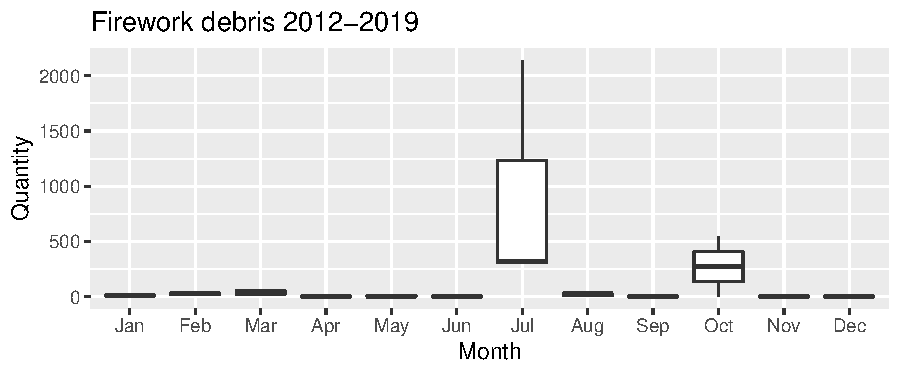
\includegraphics[width=\maxwidth]{figure/unnamed-chunk-14-1} 
\begin{kframe}\begin{verbatim}
## $tm
##    Material Description                           ItemName   vSize vColor
## 1                 CLOTH                 Clothing and Shoes    6336      1
## 2                 CLOTH                      Fabric pieces    6172      1
## 3                 CLOTH                Gloves (non-rubber)     653      1
## 4                 CLOTH                               <NA>   15168      4
## 5                 CLOTH                     Towels or rags    2007      1
## 6          FISHING GEAR                   Buoys and floats    2397      1
## 7          FISHING GEAR       Crab/Lobster/Fish trap parts    1185      1
## 8          FISHING GEAR            Fishing lures and lines    6391      1
## 9          FISHING GEAR                       Fishing nets     104      1
## 10         FISHING GEAR                               <NA>   67442      6
## 11         FISHING GEAR    Plastic rope / Small Net Pieces   52221      1
## 12         FISHING GEAR     Rope or Net Pieces (non-nylon)    5144      1
## 13                GLASS                       Glass Bottle   23298      1
## 14                GLASS                    Glass fragments     907      1
## 15                GLASS                         Glass Jars    1603      1
## 16                GLASS                               <NA>   25808      3
## 17                METAL                       Aerosol cans    5201      1
## 18                METAL               Aluminum or tin cans   31606      1
## 19                METAL    Batteries (acidic and alkaline)     248      1
## 20                METAL                  Metal Bottle Caps   12901      1
## 21                METAL                    Metal fragments     738      1
## 22                METAL                               <NA>   50694      5
## 23          OTHER ITEMS                               <NA>   62649      2
## 24          OTHER ITEMS                              Other   50223      1
## 25          OTHER ITEMS                          Test Item   12426      1
## 26       PAPER & LUMBER              Food wrappers (paper)   23690      1
## 27       PAPER & LUMBER          Lumber/Building Materials    9335      1
## 28       PAPER & LUMBER                               <NA>   83006      6
## 29       PAPER & LUMBER                            Pallets     579      1
## 30       PAPER & LUMBER                Paper and Cardboard   43116      1
## 31       PAPER & LUMBER                         Paper Bags    5659      1
## 32       PAPER & LUMBER                         Paper Cups     627      1
## 33              PLASTIC                   Balloons - Mylar    8993      1
## 34              PLASTIC                   Beverage Bottles   56296      1
## 35              PLASTIC           Bottle or Container Caps   67807      1
## 36              PLASTIC  Chemicals and chemical containers      40      1
## 37              PLASTIC                         Cigar Tips    1734      1
## 38              PLASTIC     Cigarette or tobacco packaging    3728      1
## 39              PLASTIC                         Cigarettes  389889      1
## 40              PLASTIC      Disposable cigarette lighters    7234      1
## 41              PLASTIC                     Film fragments    2591      1
## 42              PLASTIC                          Fireworks    3565      1
## 43              PLASTIC                     Foam fragments    4481      1
## 44              PLASTIC               Foam or Plastic Cups   27031      1
## 45              PLASTIC                      Food Wrappers  113817      1
## 46              PLASTIC             Hard plastic fragments    7935      1
## 47              PLASTIC                               <NA> 1098985     25
## 48              PLASTIC Non-food related plastic packaging    1737      1
## 49              PLASTIC           Other Jugs or Containers   12904      1
## 50              PLASTIC             Personal care products    8154      1
## 51              PLASTIC                       Plastic Bags   45711      1
## 52              PLASTIC          Plastic or Foam Fragments  273536      1
## 53              PLASTIC                   Plastic Utensils   24673      1
## 54              PLASTIC                      Rubber Gloves    2114      1
## 55              PLASTIC                     Six-pack rings    1420      1
## 56              PLASTIC                             Straws   27857      1
## 57              PLASTIC                Styrofoam packaging    3474      1
## 58              PLASTIC                     Toys (plastic)    2264      1
## 59               RUBBER                         Flip-flops    4661      1
## 60               RUBBER                     Latex balloons      84      1
## 61               RUBBER                               <NA>  106823      5
## 62               RUBBER                   Rubber fragments     335      1
## 63               RUBBER                      Rubber Gloves     155      1
## 64               RUBBER                              Tires  101588      1
##     stdErr vColorValue level        x0          y0            w           h
## 1     6336          NA     2 0.8531943 0.000000000 0.0613238944 0.068397960
## 2     6172          NA     2 0.9145182 0.000000000 0.0597365966 0.068397960
## 3      653          NA     2 0.9742548 0.000000000 0.0257451956 0.016790928
## 4    15168          NA     1 0.8531943 0.000000000 0.1468056866 0.068397960
## 5     2007          NA     2 0.9742548 0.016790928 0.0257451956 0.051607032
## 6     2397          NA     2 0.9644487 0.719882250 0.0355512621 0.044634504
## 7     1185          NA     2 0.9644487 0.695879799 0.0326828903 0.024002452
## 8     6391          NA     2 0.8531943 0.695879799 0.0616408346 0.068636956
## 9      104          NA     2 0.9971316 0.695879799 0.0028683718 0.024002452
## 10   67442          NA     1 0.8531943 0.695879799 0.1468056866 0.304120201
## 11   52221          NA     2 0.8531943 0.764516755 0.1468056866 0.235483245
## 12    5144          NA     2 0.9148351 0.695879799 0.0496135899 0.068636956
## 13   23298          NA     2 0.8531943 0.068397960 0.1325278552 0.116377542
## 14     907          NA     2 0.9857222 0.068397960 0.0142778314 0.042053558
## 15    1603          NA     2 0.9857222 0.110451518 0.0142778314 0.074323984
## 16   25808          NA     1 0.8531943 0.068397960 0.1468056866 0.116377542
## 17    5201          NA     2 0.9524158 0.198492909 0.0475841776 0.072357240
## 18   31606          NA     2 0.8531943 0.270850149 0.1468056866 0.142522806
## 19     248          NA     2 0.9880316 0.184775502 0.0119684341 0.013717408
## 20   12901          NA     2 0.8531943 0.184775502 0.0992215089 0.086074648
## 21     738          NA     2 0.9524158 0.184775502 0.0356157435 0.013717408
## 22   50694          NA     1 0.8531943 0.184775502 0.1468056866 0.228597454
## 23   62649          NA     1 0.8531943 0.413372956 0.1468056866 0.282506843
## 24   50223          NA     2 0.8531943 0.469406253 0.1468056866 0.226473546
## 25   12426          NA     2 0.8531943 0.413372956 0.1468056866 0.056033297
## 26   23690          NA     2 0.6739071 0.000000000 0.1064756875 0.147289679
## 27    9335          NA     2 0.7803827 0.062416274 0.0728115719 0.084873404
## 28   83006          NA     1 0.4801204 0.000000000 0.3730739096 0.147289679
## 29     579          NA     2 0.8404032 0.000000000 0.0127910788 0.029966022
## 30   43116          NA     2 0.4801204 0.000000000 0.1937866502 0.147289679
## 31    5659          NA     2 0.7803827 0.000000000 0.0600204931 0.062416274
## 32     627          NA     2 0.8404032 0.029966022 0.0127910788 0.032450252
## 33    8993          NA     2 0.6459880 0.269153750 0.0873999284 0.068116327
## 34   56296          NA     2 0.6998035 0.534216090 0.1533908431 0.242960577
## 35   67807          NA     2 0.5150484 0.534216090 0.1847550962 0.242960577
## 36      40          NA     2 0.8523133 0.147289679 0.0008809984 0.030056788
## 37    1734          NA     2 0.8210379 0.177346466 0.0321564428 0.035697582
## 38    3728          NA     2 0.7333879 0.213044048 0.0414821483 0.059493891
## 39  389889          NA     2 0.0000000 0.498869692 0.5150483741 0.501130308
## 40    7234          NA     2 0.7333879 0.272537939 0.0739803294 0.064732138
## 41    2591          NA     2 0.7333879 0.177952479 0.0488790011 0.035091570
## 42    3565          NA     2 0.7748701 0.213044048 0.0396684170 0.059493891
## 43    4481          NA     2 0.8073682 0.272537939 0.0458260791 0.064732138
## 44   27031          NA     2 0.6686979 0.337270077 0.1844964097 0.096991104
## 45  113817          NA     2 0.5150484 0.777176668 0.3381459393 0.222823332
## 46    7935          NA     2 0.6459880 0.147289679 0.0873999284 0.060102642
## 47 1098985          NA     1 0.0000000 0.147289679 0.8531943134 0.852710321
## 48    1737          NA     2 0.7822669 0.147289679 0.0387709646 0.029658619
## 49   12904          NA     2 0.5150484 0.147289679 0.1309396025 0.065239563
## 50    8154          NA     2 0.6459880 0.207392320 0.0873999284 0.061761429
## 51   45711          NA     2 0.5150484 0.337270077 0.1536495297 0.196946013
## 52  273536          NA     2 0.0000000 0.147289679 0.5150483741 0.351580013
## 53   24673          NA     2 0.5150484 0.212529242 0.1309396025 0.124740835
## 54    2114          NA     2 0.7822669 0.176948297 0.0387709646 0.036095751
## 55    1420          NA     2 0.8210379 0.147289679 0.0312754443 0.030056788
## 56   27857          NA     2 0.6686979 0.434261181 0.1844964097 0.099954910
## 57    3474          NA     2 0.8145385 0.213044048 0.0386558431 0.059493891
## 58    2264          NA     2 0.7333879 0.147289679 0.0488790011 0.030662800
## 59    4661          NA     2 0.4565915 0.016149814 0.0235289246 0.131139865
## 60      84          NA     2 0.4703235 0.000000000 0.0097968867 0.005676085
## 61  106823          NA     1 0.0000000 0.000000000 0.4801204039 0.147289679
## 62     335          NA     2 0.4565915 0.000000000 0.0137320379 0.016149814
## 63     155          NA     2 0.4703235 0.005676085 0.0097968867 0.010473729
## 64  101588          NA     2 0.0000000 0.000000000 0.4565914792 0.147289679
##      color
## 1  #C08446
## 2  #B78933
## 3  #BC863D
## 4  #D3A362
## 5  #B38B2B
## 6  #00A6AB
## 7  #00A89E
## 8  #00A7A7
## 9  #00A899
## 10 #00C1BA
## 11 #00A7A2
## 12 #00A894
## 13 #CA71BF
## 14 #D26FB0
## 15 #CE6FB8
## 16 #E68ECF
## 17 #7A9C28
## 18 #8D9813
## 19 #809B21
## 20 #93960F
## 21 #87991A
## 22 #A1B453
## 23 #5BB5E2
## 24 #009EC8
## 25 #3799CF
## 26 #D07871
## 27 #D47481
## 28 #EC929B
## 29 #D27777
## 30 #D57387
## 31 #D3757D
## 32 #D5728D
## 33 #44A352
## 34 #36A459
## 35 #22A560
## 36 #00A666
## 37 #00A66D
## 38 #3DA456
## 39 #2CA55D
## 40 #11A664
## 41 #00A66A
## 42 #00A770
## 43 #41A354
## 44 #34A45A
## 45 #20A561
## 46 #00A668
## 47 #53BF82
## 48 #00A76E
## 49 #39A458
## 50 #27A55E
## 51 #0BA665
## 52 #00A66B
## 53 #00A772
## 54 #40A454
## 55 #30A55B
## 56 #19A562
## 57 #00A669
## 58 #00A770
## 59 #AA7ED3
## 60 #9585D6
## 61 #B79FEB
## 62 #A480D4
## 63 #8D88D7
## 64 #9D83D5
## 
## $type
## [1] "index"
## 
## $vSize
## [1] "Quantity"
## 
## $vColor
## [1] NA
## 
## $stdErr
## [1] "Quantity"
## 
## $algorithm
## [1] "pivotSize"
## 
## $vpCoorX
## [1] 0.02812148 0.97187852
## 
## $vpCoorY
## [1] 0.01406074 0.93593926
## 
## $aspRatio
## [1] 1.023733
## 
## $range
## [1] NA
## 
## $mapping
## [1] NA NA NA
## 
## $draw
## [1] TRUE
## null device 
##           1
\end{verbatim}
\end{kframe}
\end{knitrout}
Cigarettes are the most common item recorded. Perhaps some of the debris is not actually from the sea, but rather from people littering by the coastline? Does debris littered on the coastline end up in the oceans?

We have locational data, so lets check for any geographical observation bias.
\begin{knitrout}
\definecolor{shadecolor}{rgb}{0.969, 0.969, 0.969}\color{fgcolor}\begin{kframe}


{\ttfamily\noindent\color{warningcolor}{\#\# Warning: Computation failed in `stat\_binhex()`:\\\#\# Package `hexbin` required for `stat\_binhex`.\\\#\# Please install and try again.}}\end{kframe}
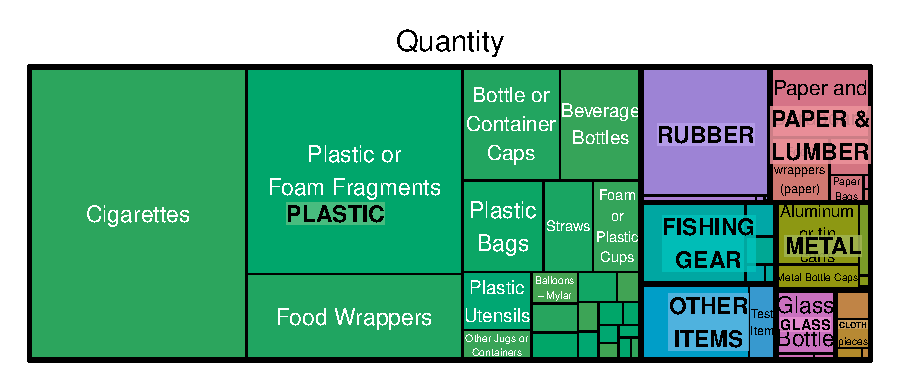
\includegraphics[width=\maxwidth]{figure/unnamed-chunk-15-1} 

\end{knitrout}
There seems to be a strong bias towards North America in our dataset. We will try a logarithmic plot to see things more clearly:
\begin{knitrout}
\definecolor{shadecolor}{rgb}{0.969, 0.969, 0.969}\color{fgcolor}\begin{kframe}


{\ttfamily\noindent\color{warningcolor}{\#\# Warning: Computation failed in `stat\_binhex()`:\\\#\# Package `hexbin` required for `stat\_binhex`.\\\#\# Please install and try again.}}\end{kframe}
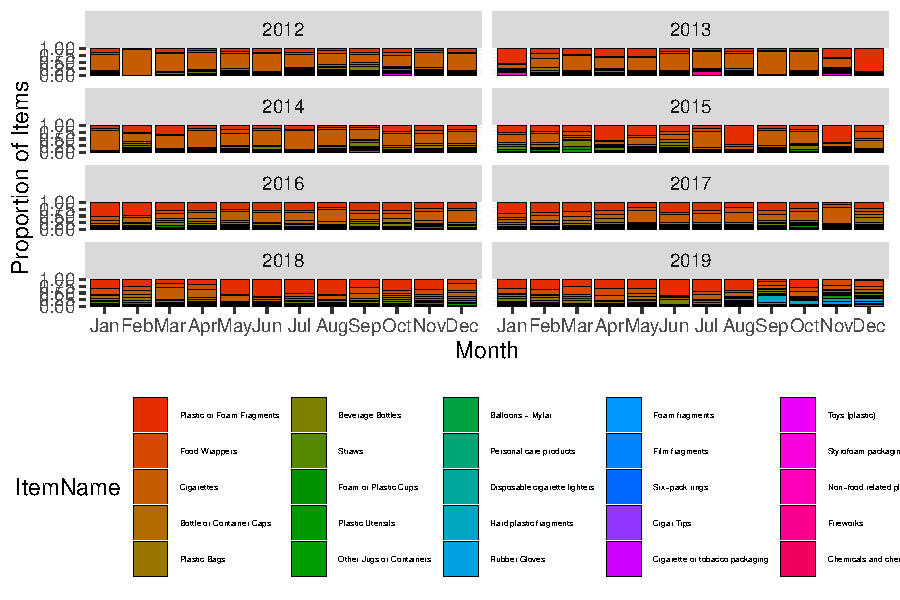
\includegraphics[width=\maxwidth]{figure/unnamed-chunk-16-1} 

\end{knitrout}

We need to know how reliable the location data is. I'm going to filter for "united kingdom" in the location field and plot the raw coordinates.
\begin{knitrout}
\definecolor{shadecolor}{rgb}{0.969, 0.969, 0.969}\color{fgcolor}
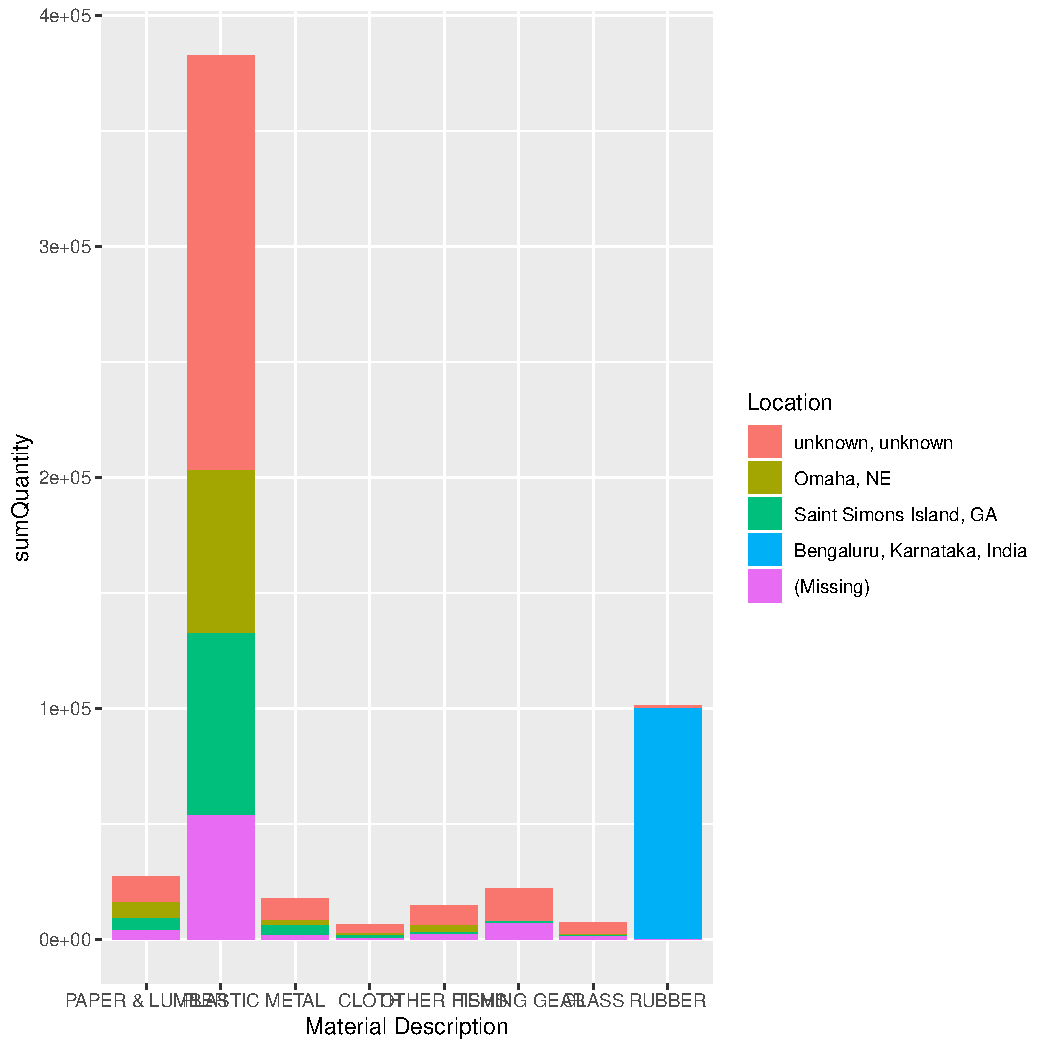
\includegraphics[width=\maxwidth]{figure/unnamed-chunk-17-1} 

\end{knitrout}
We have a outliers here. Maybe a difference in standards used for Longitude and Latitude? Some systems put the Latitude origin close to the UK.

Questions
Distribution of plastic by location.
Are the distributions of plastic fairly constant for the locations with the most observations? Let's look:
\begin{knitrout}
\definecolor{shadecolor}{rgb}{0.969, 0.969, 0.969}\color{fgcolor}
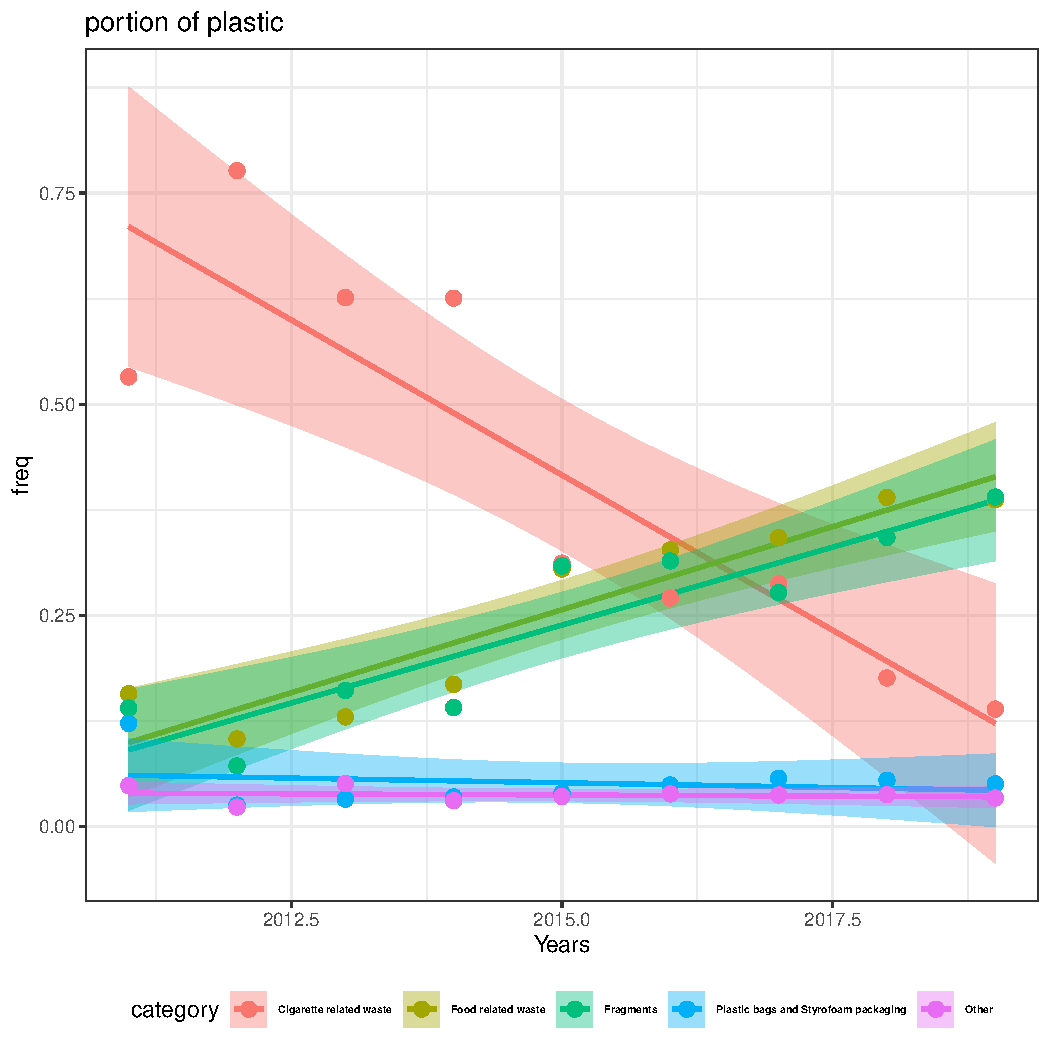
\includegraphics[width=\maxwidth]{figure/unnamed-chunk-18-1} 

\end{knitrout}
We see that the Location "unknown" has the most plastic... note that this is distinct from "(Missing)", which was our original NA values. Maybe we should merge these.

Question: Are observed plastic item proportions time invariant?

\begin{knitrout}
\definecolor{shadecolor}{rgb}{0.969, 0.969, 0.969}\color{fgcolor}
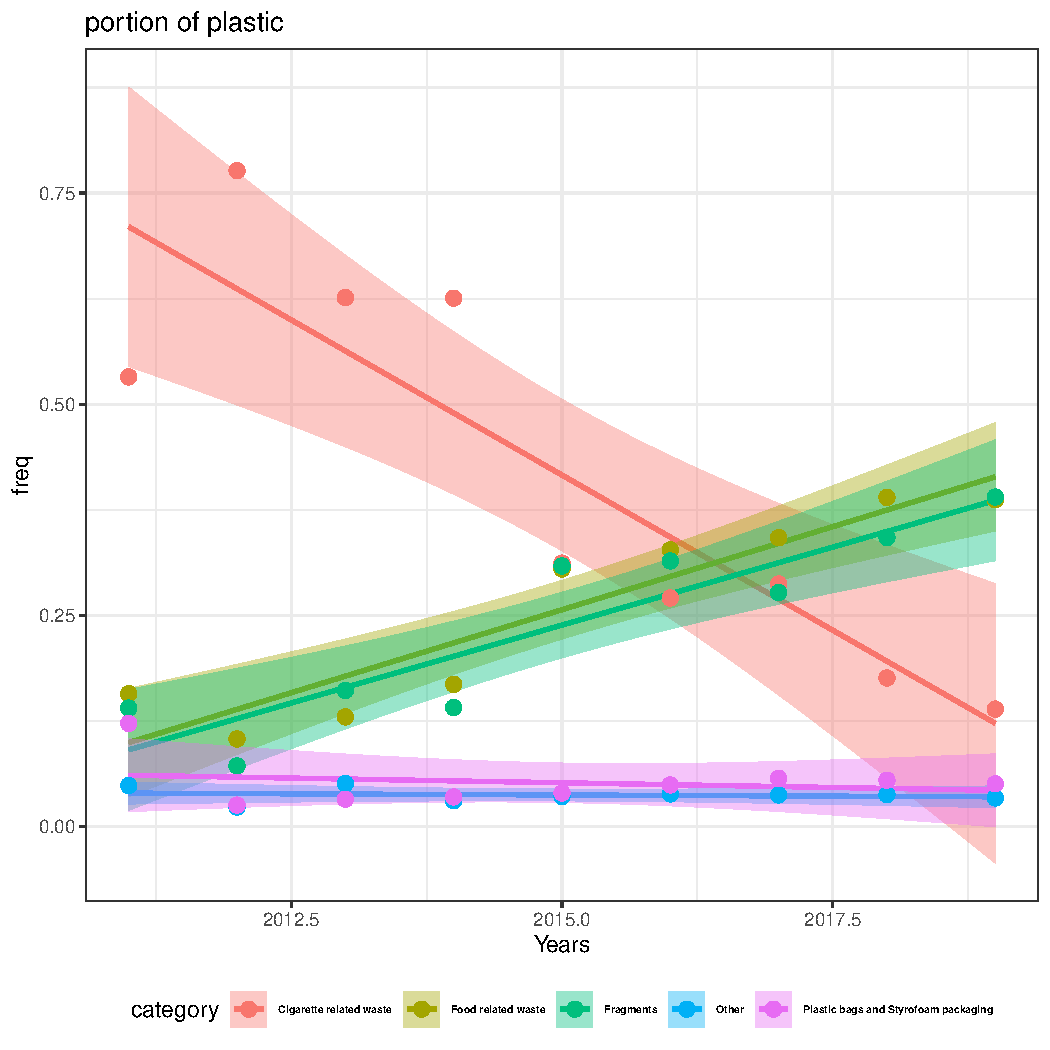
\includegraphics[width=\maxwidth]{figure/unnamed-chunk-19-1} 
\begin{kframe}

{\ttfamily\noindent\color{warningcolor}{\#\# Warning in grDevices::png(..., res = dpi, units = "{}in"{}): unable to open file 'plots/pastic\_debris\_plot.png' for writing}}

{\ttfamily\noindent\color{warningcolor}{\#\# Warning in grDevices::png(..., res = dpi, units = "{}in"{}): opening device failed}}

{\ttfamily\noindent\bfseries\color{errorcolor}{\#\# Error in grDevices::png(..., res = dpi, units = "{}in"{}): unable to start png() device}}\end{kframe}
\end{knitrout}


4th July and Firework link? (Karen's Idea)
\begin{knitrout}
\definecolor{shadecolor}{rgb}{0.969, 0.969, 0.969}\color{fgcolor}
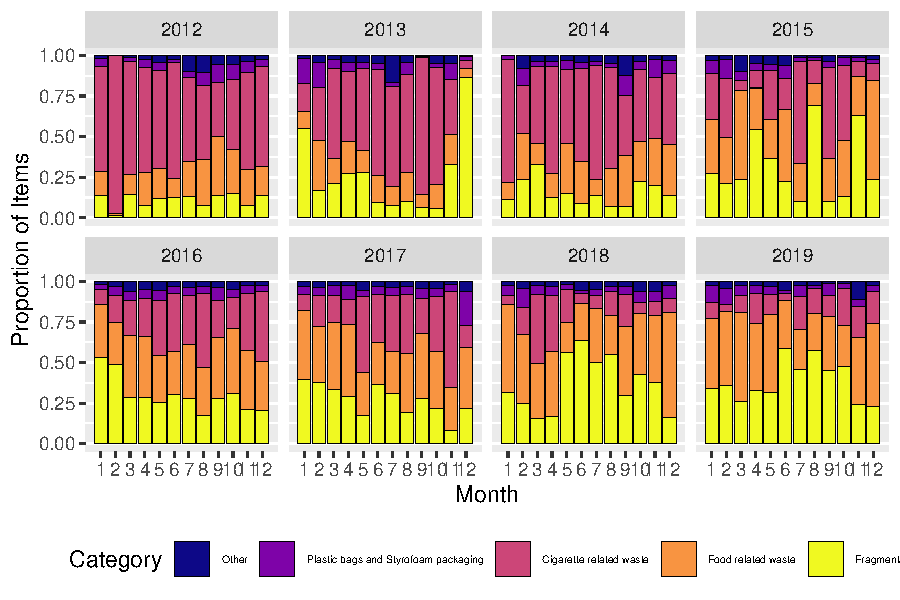
\includegraphics[width=\maxwidth]{figure/unnamed-chunk-20-1} 
\begin{kframe}

{\ttfamily\noindent\itshape\color{messagecolor}{\#\# Saving 7 x 7 in image}}

{\ttfamily\noindent\color{warningcolor}{\#\# Warning in grDevices::png(..., res = dpi, units = "{}in"{}): unable to open file 'plots/fireworks.png' for writing}}

{\ttfamily\noindent\color{warningcolor}{\#\# Warning in grDevices::png(..., res = dpi, units = "{}in"{}): opening device failed}}

{\ttfamily\noindent\bfseries\color{errorcolor}{\#\# Error in grDevices::png(..., res = dpi, units = "{}in"{}): unable to start png() device}}\end{kframe}
\end{knitrout}

\begin{knitrout}
\definecolor{shadecolor}{rgb}{0.969, 0.969, 0.969}\color{fgcolor}
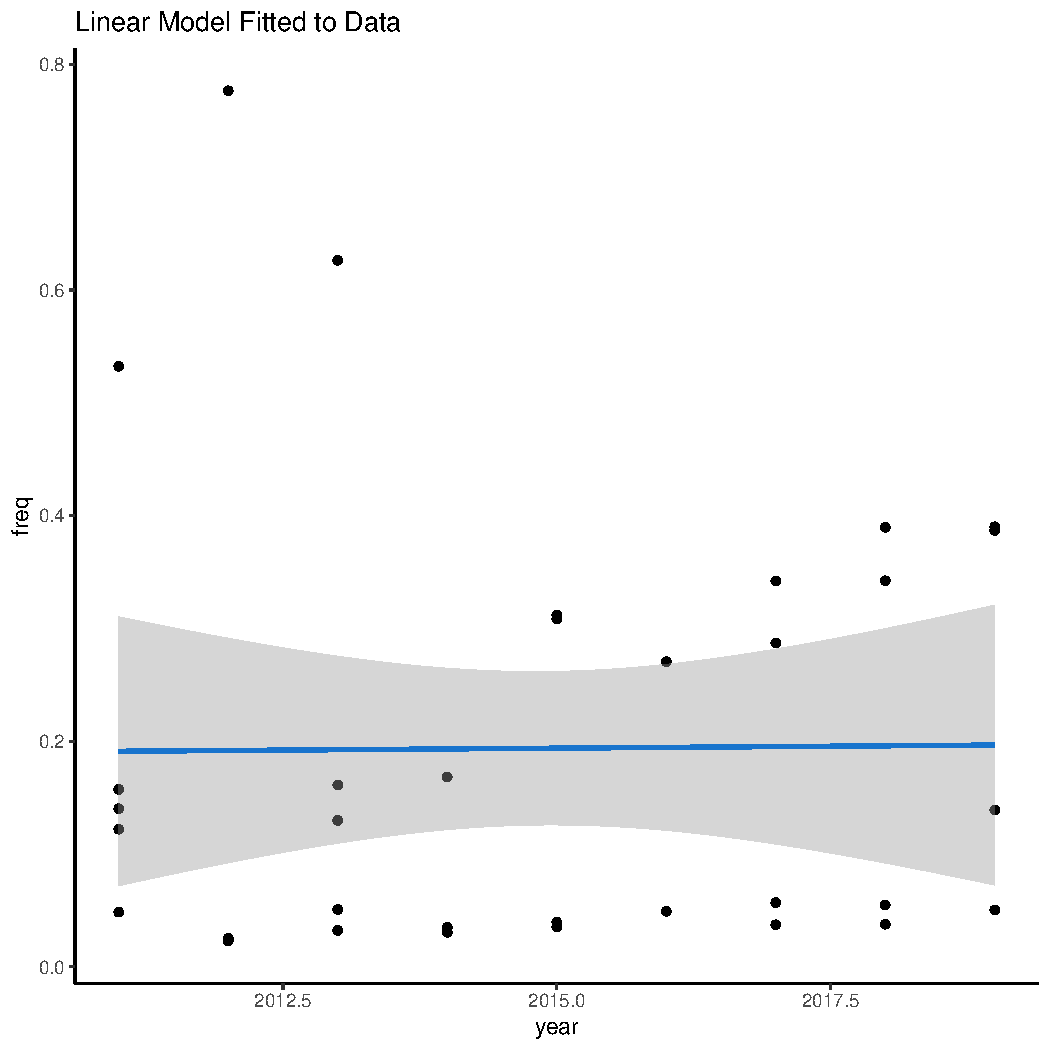
\includegraphics[width=\maxwidth]{figure/unnamed-chunk-21-1} 

\end{knitrout}

\begin{knitrout}
\definecolor{shadecolor}{rgb}{0.969, 0.969, 0.969}\color{fgcolor}
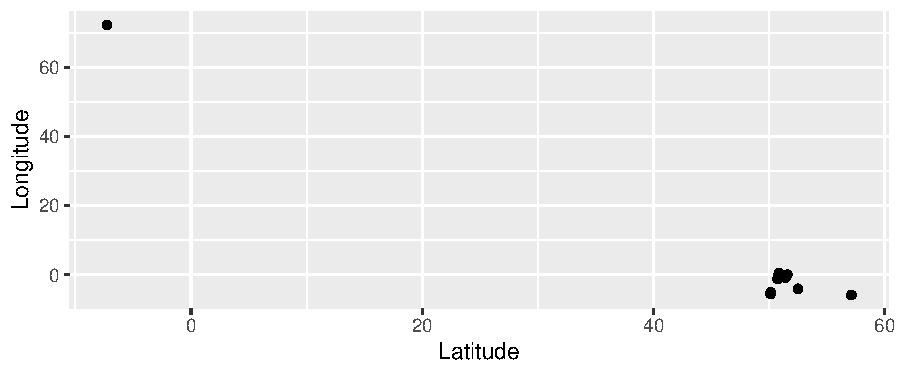
\includegraphics[width=\maxwidth]{figure/unnamed-chunk-22-1} 
\begin{kframe}

{\ttfamily\noindent\itshape\color{messagecolor}{\#\# Saving 7 x 7 in image}}

{\ttfamily\noindent\color{warningcolor}{\#\# Warning in grDevices::png(..., res = dpi, units = "{}in"{}): unable to open file 'plots/observations.png' for writing}}

{\ttfamily\noindent\color{warningcolor}{\#\# Warning in grDevices::png(..., res = dpi, units = "{}in"{}): opening device failed}}

{\ttfamily\noindent\bfseries\color{errorcolor}{\#\# Error in grDevices::png(..., res = dpi, units = "{}in"{}): unable to start png() device}}\end{kframe}
\end{knitrout}

Recategorisation
\begin{knitrout}
\definecolor{shadecolor}{rgb}{0.969, 0.969, 0.969}\color{fgcolor}
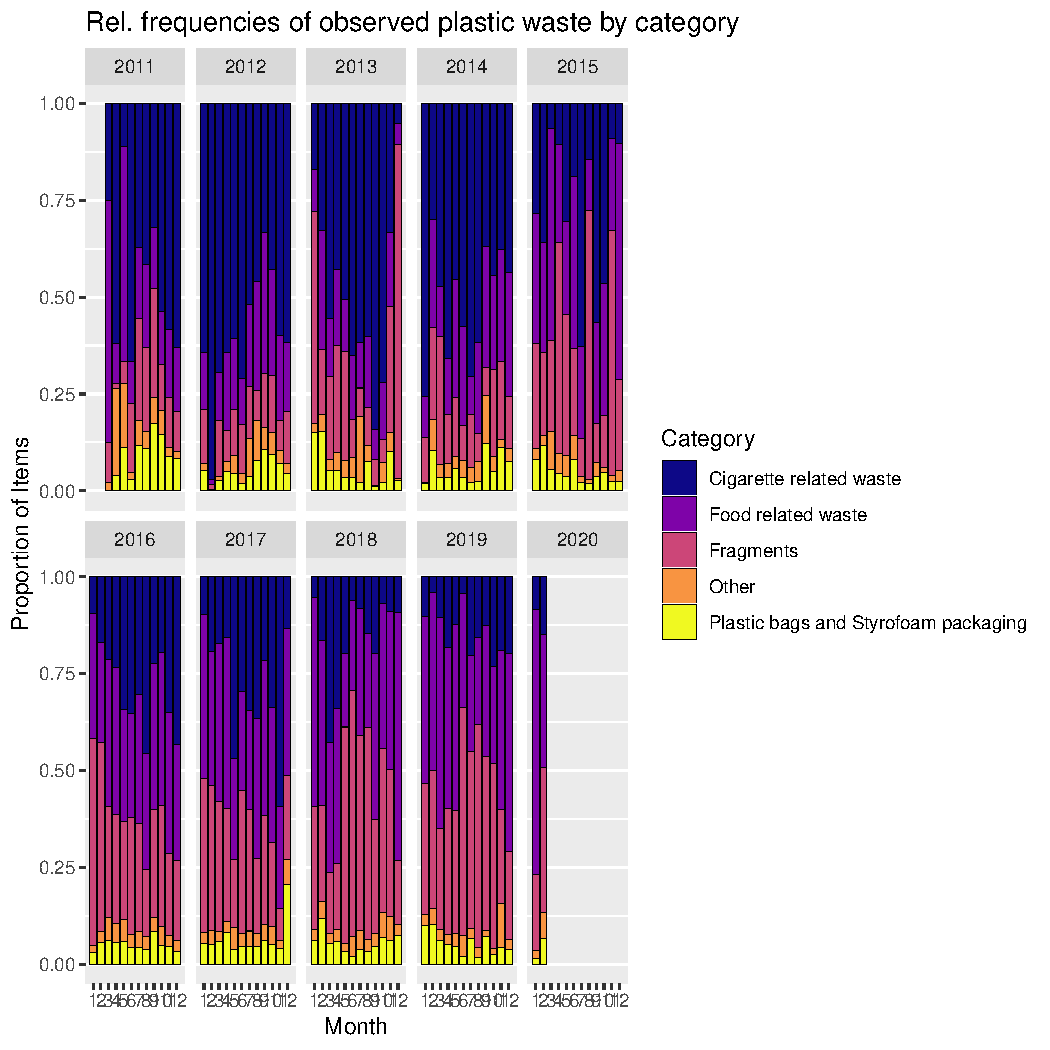
\includegraphics[width=\maxwidth]{figure/unnamed-chunk-23-1} 

\end{knitrout}


After the issues with the dataset that were identified in the section above, it was decided that it would be best to transform the dataset in the following ways:
\begin{itemize}
\item reclassified some labels because variation was too high (there were too many labels)
\item The values of the missing data were removed.
\item It was decided that subsets that were not needed were removed while retaining the necessary subsets.

\end{itemize}

\section{Exploration}

Here we describe the things we found... 

\subsection{Proportion Trends}
How pollutant proportions change over time.

Cigarette butts proportions and raw counts decrease over time: possibly less people smoking, or moving to vaping

General pollution count going down over time?

Old pollutants fall away (cigarette butts) but new ones are introduced

\subsection{Event-Driven Pollution}

Fireworks found in July and North-America only: possibly 4th July celebrations

\subsection{Location-Driven Pollution}

Rubber found in Indoneasia only: possibly a recording bias.

Certain classes are found in certain regions only: not because they don't exist elsewhere but because of recording bias focus in those areas


\subsection{Item Pairing} 
(e.g. are 6-pack beer rings observed at the same time as fireworks? )


\section{Predictive Modelling}
The authors of this report built a model to predict the proportion of plastics given Month and Location. This would give more accurate predictions as opposed to a simple linear model, given we know that event-driven pollution will determine different pollutants are different times.

\subsection{Description of Model}

Georgios' script
\begin{knitrout}
\definecolor{shadecolor}{rgb}{0.969, 0.969, 0.969}\color{fgcolor}\begin{kframe}
\begin{alltt}
\hlstd{plasticN} \hlkwb{<-} \hlstd{plastic} \hlopt
  \hlkwd{mutate}\hlstd{(}\hlkwc{year} \hlstd{=} \hlkwd{as.integer}\hlstd{(}\hlkwd{year}\hlstd{(Time)))} \hlopt
  \hlkwd{filter}\hlstd{(year} \hlopt{>} \hlnum{2010}\hlstd{)} \hlopt
  \hlkwd{group_by}\hlstd{(year, category)} \hlopt
  \hlkwd{summarise}\hlstd{(}\hlkwc{`Total Quantity`} \hlstd{=} \hlkwd{sum}\hlstd{(Quantity))}

  \hlcom{####}
\hlkwd{library}\hlstd{(dplyr)}
\hlstd{df11N} \hlkwb{<-} \hlstd{plasticN}  \hlopt
  \hlkwd{filter}\hlstd{(year} \hlopt{==} \hlnum{2011}\hlstd{)} \hlopt
  \hlkwd{group_by}\hlstd{(year)} \hlopt
  \hlkwd{mutate}\hlstd{(}\hlkwc{freq} \hlstd{= `Total Quantity`} \hlopt{/} \hlkwd{sum}\hlstd{(`Total Quantity`))}

\hlstd{df12N} \hlkwb{<-} \hlstd{plasticN}  \hlopt
  \hlkwd{filter}\hlstd{(year} \hlopt{==} \hlnum{2012}\hlstd{)} \hlopt
  \hlkwd{group_by}\hlstd{(year)} \hlopt
  \hlkwd{mutate}\hlstd{(}\hlkwc{freq} \hlstd{= `Total Quantity`} \hlopt{/} \hlkwd{sum}\hlstd{(`Total Quantity`))}


\hlstd{df13N} \hlkwb{<-} \hlstd{plasticN}  \hlopt
  \hlkwd{filter}\hlstd{(year} \hlopt{==} \hlnum{2013}\hlstd{)} \hlopt
  \hlkwd{group_by}\hlstd{(year)} \hlopt
  \hlkwd{mutate}\hlstd{(}\hlkwc{freq} \hlstd{= `Total Quantity`} \hlopt{/} \hlkwd{sum}\hlstd{(`Total Quantity`))}


\hlstd{df14N} \hlkwb{<-} \hlstd{plasticN}  \hlopt
  \hlkwd{filter}\hlstd{(year} \hlopt{==} \hlnum{2014}\hlstd{)} \hlopt
  \hlkwd{group_by}\hlstd{(year)} \hlopt
  \hlkwd{mutate}\hlstd{(}\hlkwc{freq} \hlstd{= `Total Quantity`} \hlopt{/} \hlkwd{sum}\hlstd{(`Total Quantity`))}

\hlstd{df15N} \hlkwb{<-} \hlstd{plasticN}  \hlopt
  \hlkwd{filter}\hlstd{(year} \hlopt{==} \hlnum{2015}\hlstd{)} \hlopt
  \hlkwd{group_by}\hlstd{(year)} \hlopt
  \hlkwd{mutate}\hlstd{(}\hlkwc{freq} \hlstd{= `Total Quantity`} \hlopt{/} \hlkwd{sum}\hlstd{(`Total Quantity`))}


\hlstd{df16N} \hlkwb{<-} \hlstd{plasticN}  \hlopt
  \hlkwd{filter}\hlstd{(year} \hlopt{==} \hlnum{2016}\hlstd{)} \hlopt
  \hlkwd{group_by}\hlstd{(year)} \hlopt
  \hlkwd{mutate}\hlstd{(}\hlkwc{freq} \hlstd{= `Total Quantity`} \hlopt{/} \hlkwd{sum}\hlstd{(`Total Quantity`))}



\hlstd{df17N} \hlkwb{<-} \hlstd{plasticN}  \hlopt
  \hlkwd{filter}\hlstd{(year} \hlopt{==} \hlnum{2017}\hlstd{)} \hlopt
  \hlkwd{group_by}\hlstd{(year)} \hlopt
  \hlkwd{mutate}\hlstd{(}\hlkwc{freq} \hlstd{= `Total Quantity`} \hlopt{/} \hlkwd{sum}\hlstd{(`Total Quantity`))}


\hlstd{df18N} \hlkwb{<-} \hlstd{plasticN}  \hlopt
  \hlkwd{filter}\hlstd{(year} \hlopt{==} \hlnum{2018}\hlstd{)} \hlopt
  \hlkwd{group_by}\hlstd{(year)} \hlopt
  \hlkwd{mutate}\hlstd{(}\hlkwc{freq} \hlstd{= `Total Quantity`} \hlopt{/} \hlkwd{sum}\hlstd{(`Total Quantity`))}

\hlstd{df19N} \hlkwb{<-} \hlstd{plasticN}  \hlopt
  \hlkwd{filter}\hlstd{(year} \hlopt{==} \hlnum{2019}\hlstd{)} \hlopt
  \hlkwd{group_by}\hlstd{(year)} \hlopt
  \hlkwd{mutate}\hlstd{(}\hlkwc{freq} \hlstd{= `Total Quantity`} \hlopt{/} \hlkwd{sum}\hlstd{(`Total Quantity`))}


\hlstd{dfTotN} \hlkwb{<-} \hlkwd{rbind}\hlstd{(df11N, df12N, df13N, df14N, df15N, df16N, df17N, df18N, df19N)}

\hlcom{# plot for observing the data}
\hlstd{(time_plotfr2N} \hlkwb{<-} \hlkwd{ggplot}\hlstd{(dfTotN,} \hlkwd{aes}\hlstd{(}\hlkwc{x} \hlstd{= year,} \hlkwc{y} \hlstd{= freq,} \hlkwc{color}\hlstd{=category,} \hlkwc{fill} \hlstd{= category))} \hlopt{+}
  \hlkwd{geom_smooth}\hlstd{(}\hlkwc{method}\hlstd{=}\hlstr{"lm"}\hlstd{)} \hlopt{+}
  \hlkwd{geom_point}\hlstd{(}\hlkwc{size}\hlstd{=}\hlnum{3}\hlstd{)} \hlopt{+}
  \hlkwd{theme_bw}\hlstd{()} \hlopt{+}
  \hlkwd{xlab}\hlstd{(}\hlstr{"Years"}\hlstd{)} \hlopt{+}
  \hlkwd{ylab}\hlstd{(}\hlstr{"freq"}\hlstd{)} \hlopt{+}
  \hlkwd{ggtitle}\hlstd{(}\hlstr{"portion of plastic"}\hlstd{)} \hlopt{+}
  \hlkwd{expand_limits}\hlstd{(}\hlkwc{y}\hlstd{=}\hlnum{0}\hlstd{)} \hlopt{+}
  \hlkwd{scale_y_continuous}\hlstd{()} \hlopt{+}
  \hlkwd{scale_x_continuous}\hlstd{()}\hlopt{+}
  \hlkwd{theme}\hlstd{(}\hlkwc{legend.position}\hlstd{=}\hlstr{"bottom"}\hlstd{)}\hlopt{+}
  \hlkwd{theme}\hlstd{(}\hlkwc{legend.text} \hlstd{=} \hlkwd{element_text}\hlstd{(}\hlkwc{size}\hlstd{=}\hlnum{5}\hlstd{,} \hlkwc{face}\hlstd{=}\hlstr{"bold"}\hlstd{)))}

  \hlcom{### MODELING with new categorisation}


\hlcom{# create train and test set}
\hlstd{n} \hlkwb{<-} \hlkwd{nrow}\hlstd{(dfTotN)}  \hlcom{# Number of observations}
\hlstd{ntrain} \hlkwb{<-} \hlkwd{round}\hlstd{(n}\hlopt{*}\hlnum{0.75}\hlstd{)}  \hlcom{# 75% for training set}
\hlkwd{set.seed}\hlstd{(}\hlnum{314}\hlstd{)}    \hlcom{# Set seed for reproducible results}
\hlstd{tindex} \hlkwb{<-} \hlkwd{sample}\hlstd{(n, ntrain)}   \hlcom{# Create a random index}
\hlstd{train_dfTotN} \hlkwb{<-} \hlstd{dfTotN[tindex,]}   \hlcom{# Create training set}
\hlstd{test_dfTotN} \hlkwb{<-} \hlstd{dfTotN[}\hlopt{-}\hlstd{tindex,]}

\hlcom{#  Pr(>|t|) is the p-value, defined as the probability of observing any value equal or larger than t if H0 is true. The larger the t statistic, the smaller the p-value. Generally, we use 0.05 as the cutoff for significance; when p-values are smaller than 0.05, we reject H0. Here p is pretty big which means that there is statistically significant correlation between relative frequency and years passing by. Which basically further supports our initial hypothesis in this project. I have included a prediction on the test set but it is of no worth obviously.}


\hlcom{# linear model on train set}
\hlkwd{print}\hlstd{(}\hlstr{"train model"}\hlstd{)}
\hlkwd{set.seed}\hlstd{(}\hlnum{1234}\hlstd{)}
\hlstd{dfTot_train.modelN} \hlkwb{<-} \hlkwd{lm}\hlstd{(freq} \hlopt{~} \hlstd{year,} \hlkwc{data} \hlstd{= train_dfTotN)}
\hlkwd{summary}\hlstd{(dfTot_train.modelN)}

\hlcom{# plotting frequencies according to train data}
\hlkwd{ggplot}\hlstd{(}\hlkwc{data} \hlstd{= train_dfTotN,} \hlkwd{aes}\hlstd{(}\hlkwc{x} \hlstd{= year,} \hlkwc{y} \hlstd{= freq))} \hlopt{+}
\hlkwd{geom_point}\hlstd{()} \hlopt{+}
\hlkwd{stat_smooth}\hlstd{(}\hlkwc{method} \hlstd{=} \hlstr{"lm"}\hlstd{,} \hlkwc{col} \hlstd{=} \hlstr{"dodgerblue3"}\hlstd{)} \hlopt{+}
\hlkwd{theme}\hlstd{(}\hlkwc{panel.background} \hlstd{=} \hlkwd{element_rect}\hlstd{(}\hlkwc{fill} \hlstd{=} \hlstr{"white"}\hlstd{),}
\hlkwc{axis.line.x}\hlstd{=}\hlkwd{element_line}\hlstd{(),}
\hlkwc{axis.line.y}\hlstd{=}\hlkwd{element_line}\hlstd{())} \hlopt{+}
\hlkwd{ggtitle}\hlstd{(}\hlstr{"Linear Model Fitted to Data"}\hlstd{)}


\hlkwd{print}\hlstd{(}\hlstr{"PREDICTION"}\hlstd{)}
\hlstd{predN} \hlkwb{<-} \hlkwd{predict}\hlstd{(dfTot_train.modelN, test_dfTotN)}
\hlkwd{summary}\hlstd{(predN)}

\hlcom{# make actuals_predicteds dataframe}
\hlstd{actuals_preds} \hlkwb{<-} \hlkwd{data.frame}\hlstd{(}\hlkwd{cbind}\hlstd{(}\hlkwc{actuals}\hlstd{=test_dfTotN}\hlopt{$}\hlstd{freq,} \hlkwc{predicteds}\hlstd{=predN))}
\hlkwd{head}\hlstd{(actuals_preds)}
\hlcom{# A simple correlation between the actuals and predicted values can be used as a form of accuracy measure. A higher correlation accuracy implies that the actuals and predicted values have similar directional movement, i.e. when the actuals values increase the predicteds also increase and vice-versa.}

\hlstd{correlation_accuracy} \hlkwb{<-} \hlkwd{cor}\hlstd{(actuals_preds)}  \hlcom{# 5.31%}
\hlstd{min_max_accuracy} \hlkwb{<-} \hlkwd{mean}\hlstd{(}\hlkwd{apply}\hlstd{(actuals_preds,} \hlnum{1}\hlstd{, min)} \hlopt{/} \hlkwd{apply}\hlstd{(actuals_preds,} \hlnum{1}\hlstd{, max))}
\hlcom{# => 53.73%, min_max accuracy}
\hlstd{mape} \hlkwb{<-} \hlkwd{mean}\hlstd{(}\hlkwd{abs}\hlstd{((actuals_preds}\hlopt{$}\hlstd{predicteds} \hlopt{-} \hlstd{actuals_preds}\hlopt{$}\hlstd{actuals))}\hlopt{/}\hlstd{actuals_preds}\hlopt{$}\hlstd{actuals)}
\hlcom{# => 99.4%, mean absolute percentage deviation}
\hlcom{# Intrestingly enough min_max accuracy and mostly mean absolute percentage deviation score quite well}
\hlcom{# but still on a model that can not be trusted.}
\end{alltt}
\end{kframe}
\end{knitrout}

\subsection{Model Evaluation}


\subsection{Model Results}
Time does not impact plastic composition.

\section{Discussion}



\section{Conclusion and Future Work}\label{cdsmote1}

Our hypothesis stands/does not stand.


%Edit here 
%\blindtext[2]





\section{Project Management}\label{mgt}
\subsection{Facilities}
Group 2 communicated using a dedicated Slack Channel, Github repository and weekly 1 hour meetings before the wednesday lab.
All project documents used and the final report can be accessed from the \textit{\href{https://github.com/KarenJewell/CMM507Group2}{Public Github Repository}}

\subsection{Project Progress}
%Edit here 
%\blindtext[2]
% Pay attention to the code below including the chunk options 
% latex table generated in R 3.6.1 by xtable 1.8-4 package
% Tue Apr 07 15:23:49 2020
\begin{table}[ht]
\centering
\caption{Record of Team Meetings} 
\label{tab:one}
\begin{tabular}{llp{8cm}lllll}
  \hline
No & Date & Topic & Alex & Georgios & Karen & Roshi & Stuart \\ 
  \hline
1.00 & 2020-02-05 & Group Formation: set up communication channel in Slack and GitHub repository & yes & yes & yes & yes & yes \\ 
  2.00 & 2020-02-11 & Agreed topic of "Plastic Pollution", distributed research activity for week & yes & yes & yes & yes & yes \\ 
  3.00 & 2020-02-18 & Presented inividuals' research findings and discussed hypothesis & yes & yes & yes & yes & yes \\ 
  4.00 & 2020-02-25 & Decided on final dataset to use and hypothesis of "proportion of marine plastics pollution does not change over time" & yes & yes & yes & yes & yes \\ 
  5.00 & 2020-03-04 & Presentation draft agreed & yes & yes & yes & yes & yes \\ 
  6.00 & 2020-03-10 & Distributed section writing activity for week & yes & yes & yes & yes & yes \\ 
  7.00 & 2020-03-17 &  &  &  &  &  &  \\ 
  8.00 & 2020-03-24 &  &  &  &  &  &  \\ 
  9.00 & 2020-03-31 &  &  &  &  &  &  \\ 
  10.00 & 2020-04-07 &  &  &  &  &  &  \\ 
  11.00 & 2020-04-14 &  &  &  &  &  &  \\ 
  12.00 & 2020-04-21 &  &  &  &  &  &  \\ 
   \hline
\end{tabular}
\end{table}





\subsection{Peer-assessment}

%Edit here 
%\blindtext[2] \\


% latex table generated in R 3.6.1 by xtable 1.8-4 package
% Tue Apr 07 15:23:49 2020
\begin{table}[ht]
\centering
\caption{Peer Assessment out of 100} 
\label{tab:two}
\begin{tabular}{llllll}
  \hline
Peer.Review & Alex & Georgios & Karen & Roshi & Stuart \\ 
  \hline
Alex & 100 & 100 & 100 & 100 & 100 \\ 
  Georgios & 100 & 100 & 100 & 100 & 100 \\ 
  Karen & 100 & 100 & 100 & 100 & 100 \\ 
  Roshi & 100 & 100 & 100 & 100 & 100 \\ 
  Stuart & 100 & 100 & 100 & 100 & 100 \\ 
   \hline
\end{tabular}
\end{table}




\subsection{Section on figure referencing - keep for referencing}\label{explore}

%Edit here 
%\blindtext[2]

In this project iris was used, the dataset is made of 150 rows and four features. \\

Notice how we generate graphics within the sweave document. Check the following code, we will create a function that either finds $x^2$ or $x^3$ subject to parameters passed in the function
\begin{knitrout}
\definecolor{shadecolor}{rgb}{0.969, 0.969, 0.969}\color{fgcolor}\begin{kframe}
\begin{alltt}
\hlcom{# create a vector of doubles}
\hlstd{myNumbers} \hlkwb{<-} \hlkwd{seq}\hlstd{(}\hlkwc{from}\hlstd{=}\hlopt{-}\hlnum{1}\hlstd{,}\hlkwc{to}\hlstd{=}\hlnum{1}\hlstd{,}\hlkwc{by}\hlstd{=}\hlnum{.1}\hlstd{)}

\hlcom{# function definition}
\hlstd{toPower} \hlkwb{<-} \hlkwa{function} \hlstd{(}\hlkwc{x}\hlstd{,}\hlkwc{p}\hlstd{=}\hlnum{2}\hlstd{) \{}
    \hlkwa{if} \hlstd{(p}\hlopt{==}\hlnum{2}\hlstd{)}
        \hlkwd{return} \hlstd{(x}\hlopt{*}\hlstd{x)}
    \hlkwa{else if} \hlstd{(p}\hlopt{==}\hlnum{3}\hlstd{)}
        \hlkwd{return} \hlstd{(x}\hlopt{*}\hlstd{x}\hlopt{*}\hlstd{x)}
    \hlkwd{return} \hlstd{(x}\hlopt{*}\hlstd{x)}
\hlstd{\}}

\hlcom{# call function}
\hlstd{squared} \hlkwb{<-} \hlkwd{toPower}\hlstd{(myNumbers)}
\hlstd{cubes} \hlkwb{<-} \hlkwd{toPower}\hlstd{(myNumbers,}\hlnum{3}\hlstd{)}
\end{alltt}
\end{kframe}
\end{knitrout}

An easy way to check that our function is doing the right calculation is to plot the results. The code below will generate a figure similar to Figure~\ref{fig1}: 
\begin{knitrout}
\definecolor{shadecolor}{rgb}{0.969, 0.969, 0.969}\color{fgcolor}\begin{kframe}
\begin{alltt}
\hlkwd{plot}\hlstd{(myNumbers,cubes,}\hlkwc{type}\hlstd{=}\hlstr{'b'}\hlstd{,}\hlkwc{xlab} \hlstd{=} \hlstr{'x'}\hlstd{,} \hlkwc{ylab} \hlstd{=} \hlstr{'x*x'}\hlstd{,}\hlkwc{frame}\hlstd{=}\hlnum{FALSE}\hlstd{,}\hlkwc{col}\hlstd{=}\hlstr{'blue'}\hlstd{)}
\end{alltt}
\end{kframe}
\end{knitrout}


% See carefully how we embed the R code within latex here, check captions, and figure labels 
\begin{figure}[H] %start a figure
\begin{center}

\begin{knitrout}
\definecolor{shadecolor}{rgb}{0.969, 0.969, 0.969}\color{fgcolor}
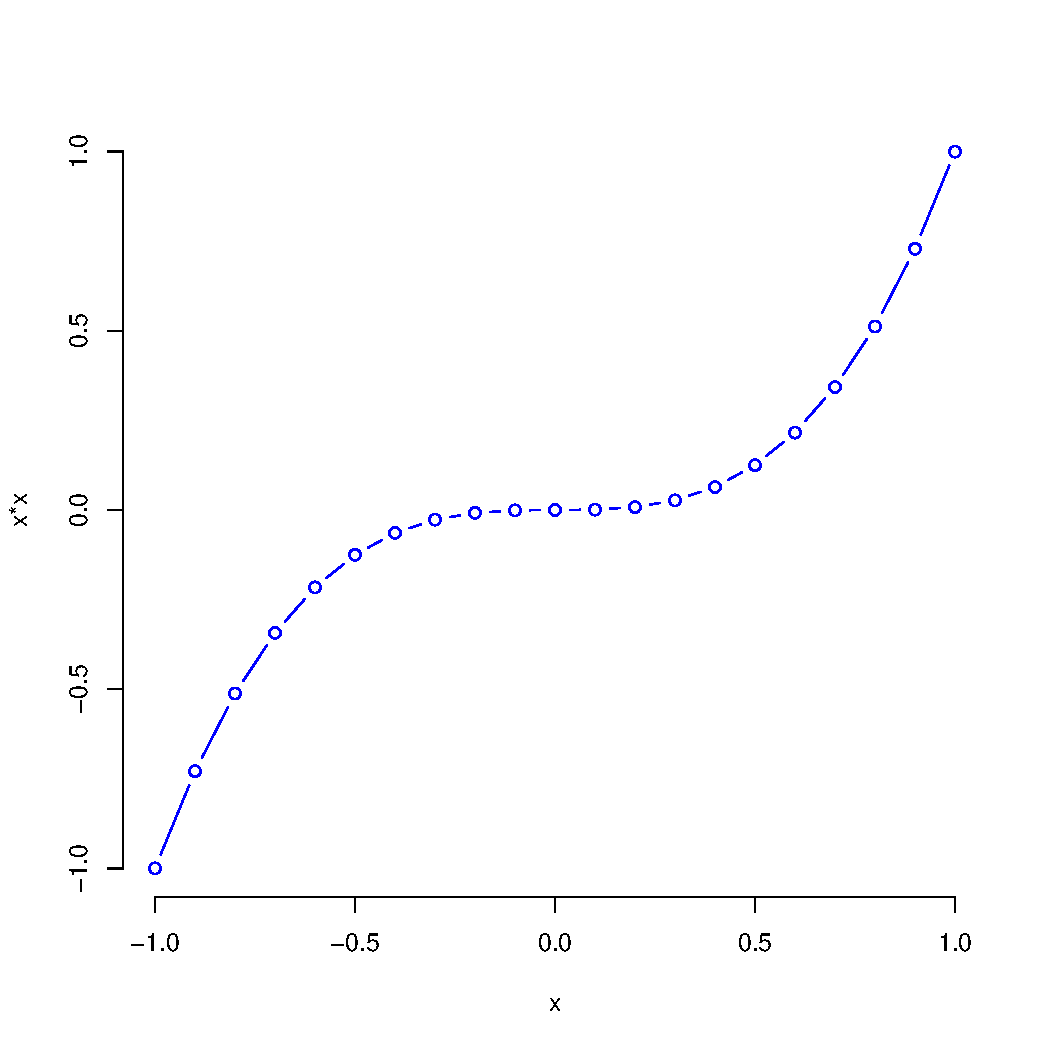
\includegraphics[width=.47\linewidth]{figure/unnamed-chunk-29-1} 

\end{knitrout}

\caption {Simple Plot of $f(x)=x^3$ Function}
\label{fig1}
\end {center}
\end {figure}




\subsection{Experiments}\label{experiments}

Now we can show how the function $f(x)=x^2$ looks like (Figure~\ref{fig2})

\begin{figure}[H] %start a figure
\begin{center}

\begin{knitrout}
\definecolor{shadecolor}{rgb}{0.969, 0.969, 0.969}\color{fgcolor}
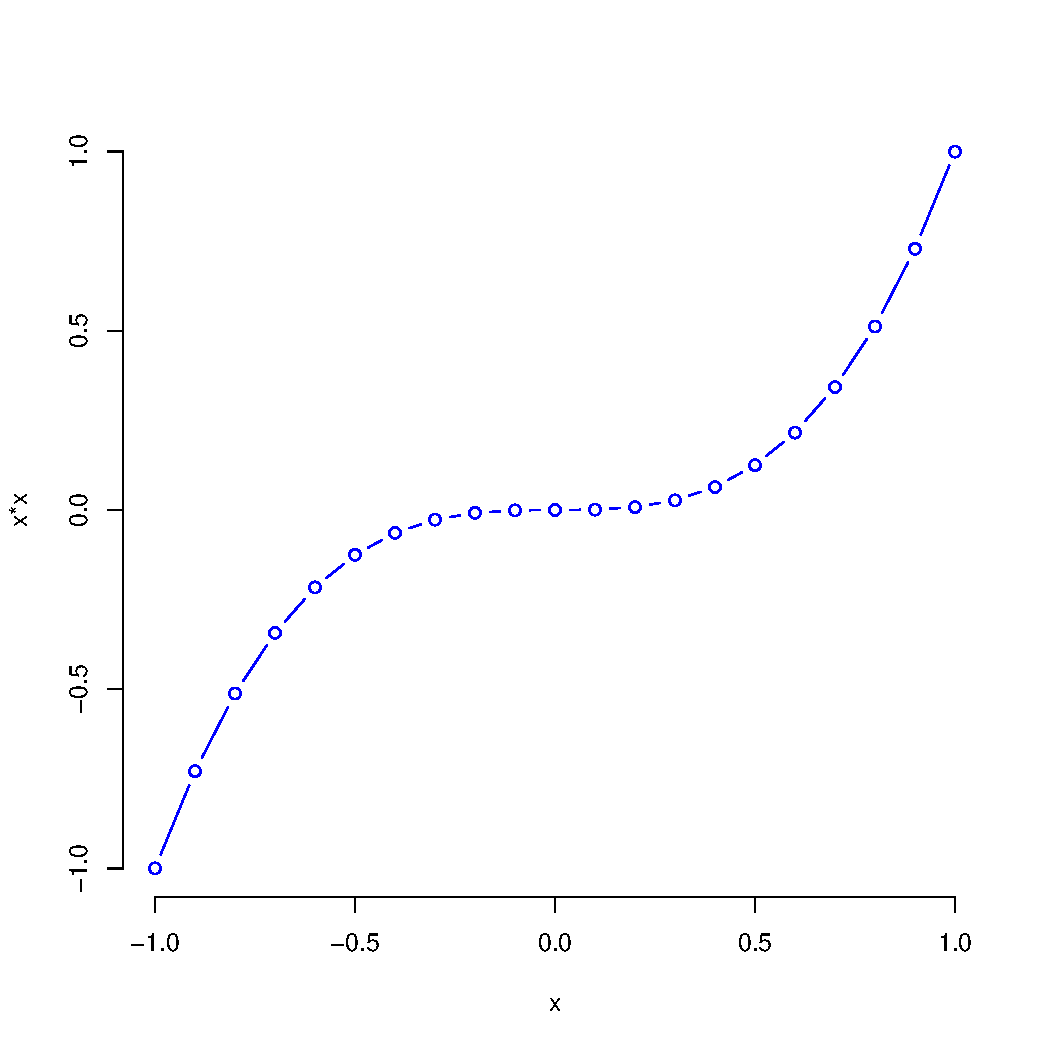
\includegraphics[width=.47\linewidth]{figure/unnamed-chunk-30-1} 

\end{knitrout}

\caption {Simple Plot of $f(x)=x^3$ Function}
\label{fig2}
\end {center}
\end {figure}

\section*{References}\label{pubs}
\printbibliography[heading =none]

\end{document}
